\documentclass[12pt]{article}

 %%%%%%%%%% LOADING PACKAGES %%%%%%%%%% 
\usepackage{amsmath, amssymb, amsfonts, bm, mathtools} % math packages
\usepackage[table]{xcolor}
\usepackage{physics}
\usepackage{graphicx}
\usepackage{parskip}
\usepackage{fancyhdr}
\usepackage{vmargin}
\usepackage{tcolorbox}
\usepackage{url}
\usepackage[utf8x]{inputenc}
\usepackage{hyperref} % to click and go to pointed place in the document
\usepackage{cancel} % for easy cancellations
\usepackage{minted} % for highlighting code
\usepackage{comment} % for multi-line commenting

 %%%%%%%%%% SET DEFAULTS %%%%%%%%%% 
\newcommand{\smallspace}{\hspace{0.5cm}}
\setcounter{secnumdepth}{0} % for avoiding the numbering
\newenvironment{sfemph}{\begin{sffamily}\begin{emph}}{\end{sffamily}\end{emph}}
 % the text inside the exercise setup will be emphasized
 % Set defaults for minted
\setminted{frame=lines,
framesep=2mm,
baselinestretch=1.2,
bgcolor=,
fontsize=\footnotesize,
linenos
}

 %%%%%%%%%% INSERT YOUR DATA HERE %%%%%%%%%% 
\title{Stock Price Prediction with Machine Learning}						
\author{Federico Berto}			 				
\date{\today}											
\newcommand{\professor}{Woo Chang Kim}
\newcommand{\studentid}{20204817}
\newcommand{\coursename}{Introduction to Financial Engineering}
\newcommand{\courseid}{IE471}
\newcommand{\firstuniversityline}{Korea Advanced Institute of Science} % first line of university name
\newcommand{\seconduniversityline}{and Technology} % split the title for better compatibility. You may modify this part

 %%%%%%%%%% TITLE PAGE SETUP %%%%%%%%%% 
\setmarginsrb{3 cm}{2.5 cm}{3 cm}{2.5 cm}{1 cm}{1.5 cm}{1 cm}{1.5 cm}
\makeatletter
\let\thetitle\@title
\let\theauthor\@author
\let\thedate\@date
\makeatother
\pagestyle{fancy}
\fancyhf{}
\renewcommand{\headrulewidth}{0.4pt}
\rhead{\theauthor}
\lhead{AI Project 1}
\chead{\raisebox{-1ex}{
\includegraphics[width = 3cm]{images/university_secondary_logo.png}}}
\cfoot{Page \thepage}

 %%%%%%%%%% MAIN DOCUMENT %%%%%%%%%% 
\begin{document}

 %%%%%%%%%% TITLE PAGE SETUP %%%%%%%%%% 
\begin{titlepage}
	\centering
    \textsc{\LARGE  \firstuniversityline \\ \smallskip \seconduniversityline}\\[1 cm]	% university Name
    
\includegraphics[scale = 0.18]{images/university_main_logo.png}\\[1.5 cm]	% university Logo
    
	\textsc{\Large \coursename}\\[0.5 cm]
	\rule{\linewidth}{0.2 mm} \\[0.4 cm]
	{ \huge \bfseries {\thetitle}}\\
	\rule{\linewidth}{0.2 mm} \\[1.5 cm]
	
	\begin{minipage}{0.5\textwidth}
		\begin{flushleft} \large
			\emph{Professor:}\\
		    \professor \\ [0.5cm]
            \emph{Course ID:}\\
            \courseid
			\end{flushleft}
			\end{minipage}~
			\begin{minipage}{0.4\textwidth}
			\begin{flushright} \large
			\emph{Student:} \\
			\theauthor \\[0.5cm]
			\emph{ID number:}\\
			\studentid \\
		\end{flushright}
	\end{minipage}\\[2 cm]
	
\end{titlepage}

 %%%%%%%%%% TABLE OF CONTENTS %%%%%%%%%% 
%% Uncomment this part
% \tableofcontents
% \incl
% \pagebreak


 %%%%%%%%%% MAIN TEXT %%%%%%%%%% 
\section{Introduction}

The goal of this report is to describe the experimental process and result for a simple stock market prediction. In particular, in the first experiment we will predict Samsung Electronics Co., Ltd stock price from 2000 to 2020 \footnote{Source: \href{https://finance.yahoo.com/quote/005930.KS/history/}{Yahoo Finance}}.\\
The prediction model is based on the Long Short-Term Memory (LSTM) \cite{hochreiter1997long} module in Figure \ref{fig:LSTM}\footnote{Source: \href{https://commons.wikimedia.org/wiki/File:LSTM_cell.svg}{Wikimedia}}, which is able to store past information of the data and is thus suitable for time series prediction.

\begin{figure}[h!]
    \centering
    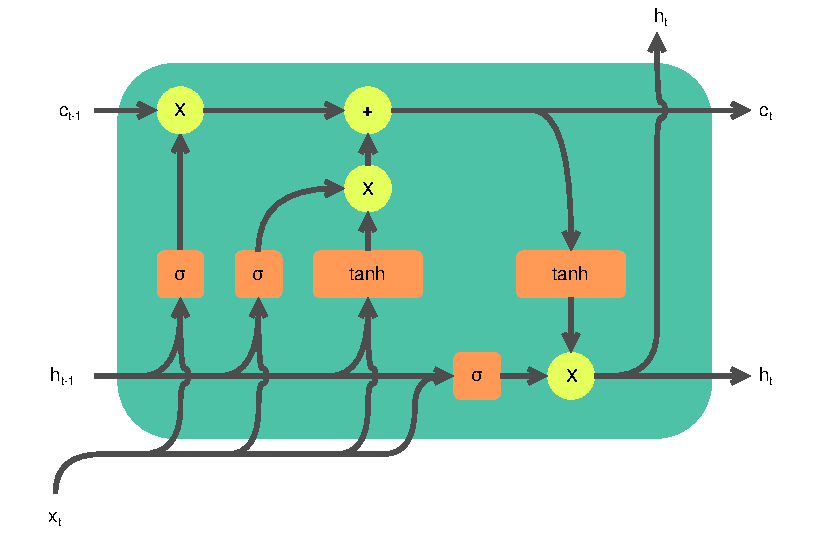
\includegraphics[width=0.7\textwidth]{images/LSTM_cell.pdf}
    \caption{LSTM cell}
    \label{fig:LSTM}
\end{figure}

Further details into the PyTorch \cite{pytorch} implementation can be found in the code, also available on the following \href{https://github.com/Juju-botu/financial-engineering-ai}{Github repository}.\footnote{Link: \href{https://github.com/Juju-botu/financial-engineering-ai}{\tt{https://github.com/Juju-botu/financial-engineering-ai}}.}

\section{Experiments with LSTM}

\subsection{Predicting Samsung's stock price}
In this section we provide the required data for the report.

\paragraph{1.} Last five data rows of the original dataset:
\rowcolors{2}{gray!25}{white}   
\begin{center}
\begin{tabular}{  l  l  l  l  l  l  l }
    \rowcolor{gray!50}
    \textbf{Date} & \textbf{High} & \textbf{Low} & \textbf{Open} & \textbf{Close} & \textbf{Volume} & \textbf{Adj Close}\\
    \hline
    \textbf{2020-12-23} & 74000.0 & 72300.0 & 72400.0 & 73900.0 & 19411326.0 & 72085.835938\\
    \textbf{2020-12-24} & 78800.0 & 74000.0 & 74100.0 & 77800.0 & 32502870.0 & 75890.093750\\
    \textbf{2020-12-28} & 80100.0 & 78200.0 & 79000.0 & 78700.0 & 40085044.0 & 76768.000000\\
    \textbf{2020-12-29} & 78900.0 & 77300.0 & 78800.0 & 78300.0 & 30339449.0 & 78300.000000\\
    \textbf{2020-12-30} & 81300.0 & 77300.0 & 77400.0 & 81000.0 & 29417421.0 & 81000.000000\\
\end{tabular}
\end{center}

\paragraph{2.} Tensor shape of training sets and test sets:

\begin{equation}
    \begin{aligned}
    &\text{Shape of Training Input Data =  } [4780, 1, 6]\\
    &\text{Shape of Training Output Data =  } [4780, 1]\\
    &\text{Shape of Test Input Data =  } [493, 1, 6]\\
    &\text{Shape of Test Input Data =  } [493, 1]\\
    \end{aligned}
\end{equation}

\paragraph{3.} Mean Squared Error every 100 epochs until 1000:

\begin{center}
\rowcolors{2}{gray!25}{white}     
\begin{tabular}{ l l }
\label{tab:loss}
    \rowcolor{gray!50}
    \textbf{Epoch} & \textbf{Loss}\\
    \hline
    100 & 0.1599 \\
     200 & 0.0392\\
     300 & 0.0143\\
     400 & 0.0099\\
     500 & 0.0071\\
     600 & 0.0051\\
     700 & 0.0037\\
     800 & 0.0026\\
     900 & 0.0019\\
     1000 & 0.0013\\
\end{tabular}
\end{center}

\paragraph{4.} Actual and predicted data: we show them graphically in Figure \ref{fig:all}, \ref{fig:train}, \ref{fig:test}.
\begin{figure}
    \centering
    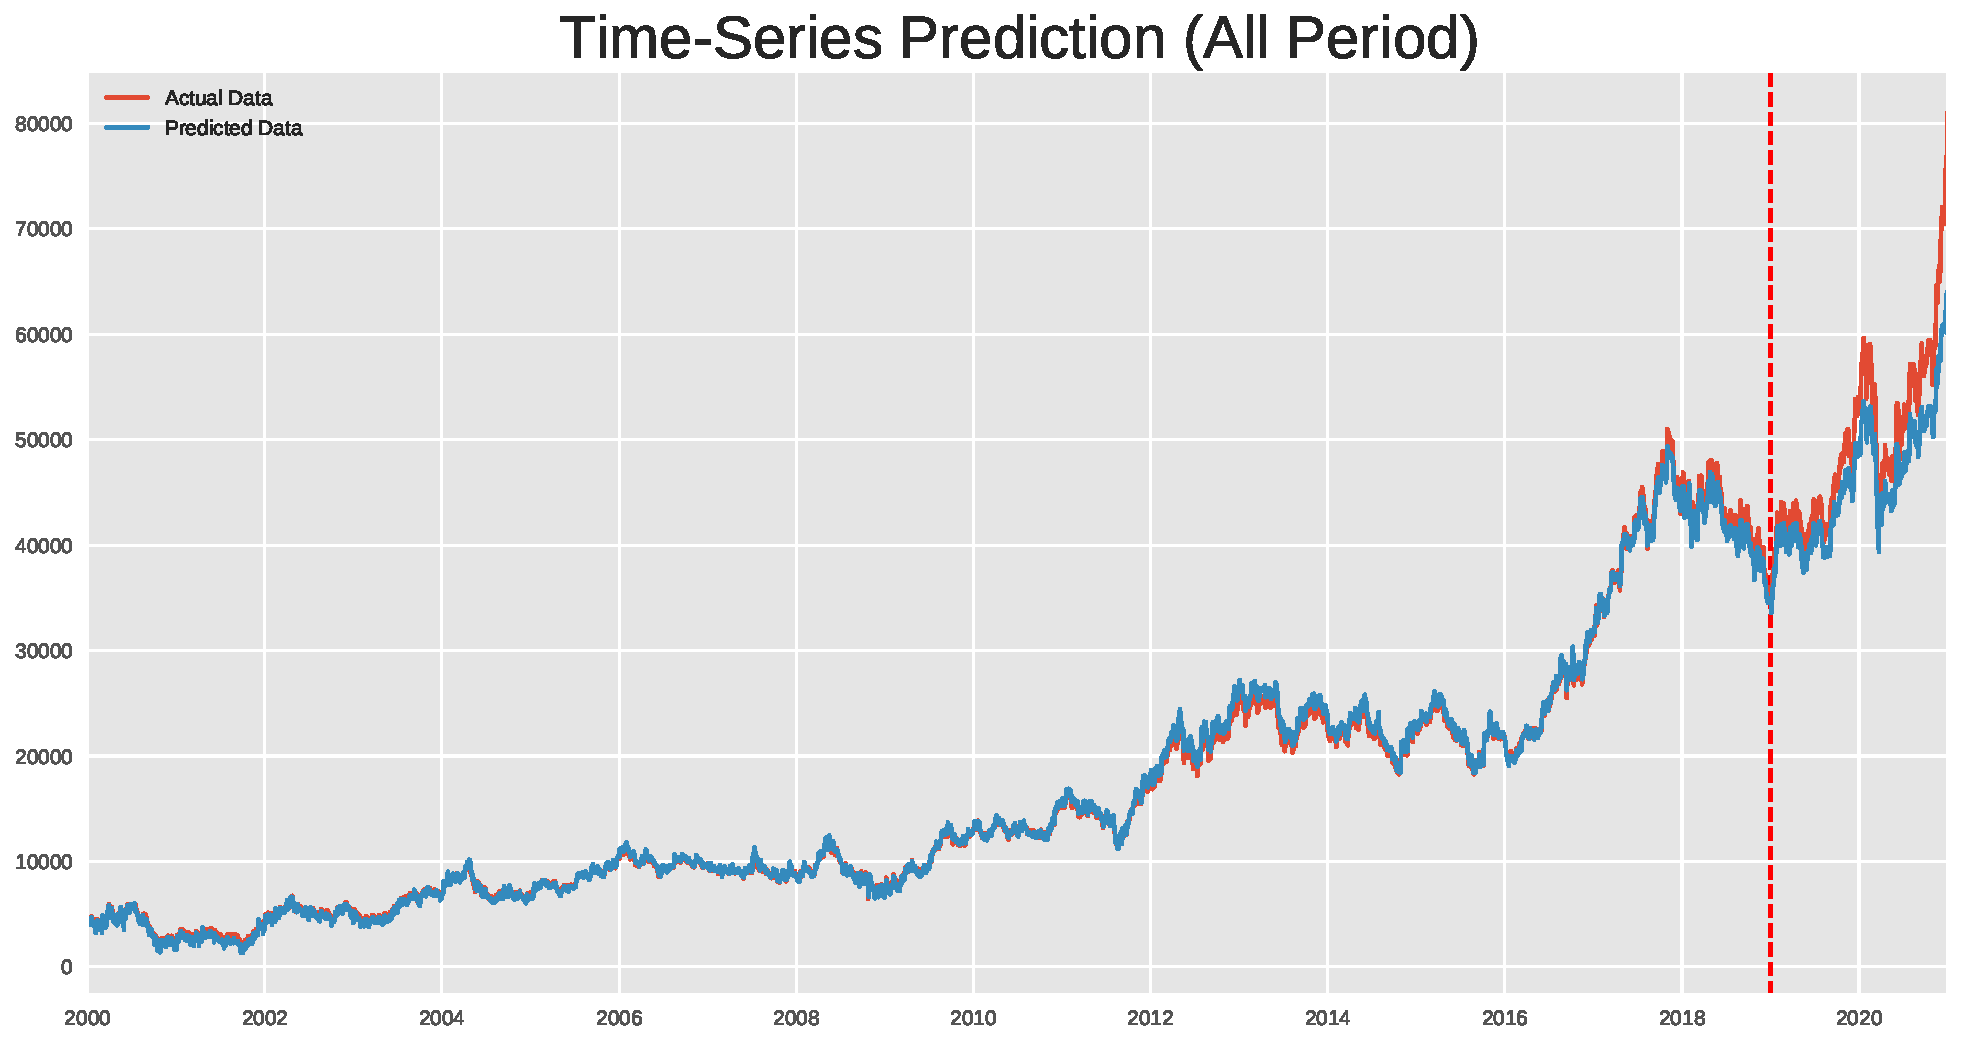
\includegraphics[width=\textwidth]{images/prediction_base_all.pdf}
    \caption{Actual and predicted adjusted closing price of Samsung's stocks the next day for all the time period}
    \label{fig:all}
\end{figure}
\begin{figure}
    \centering
    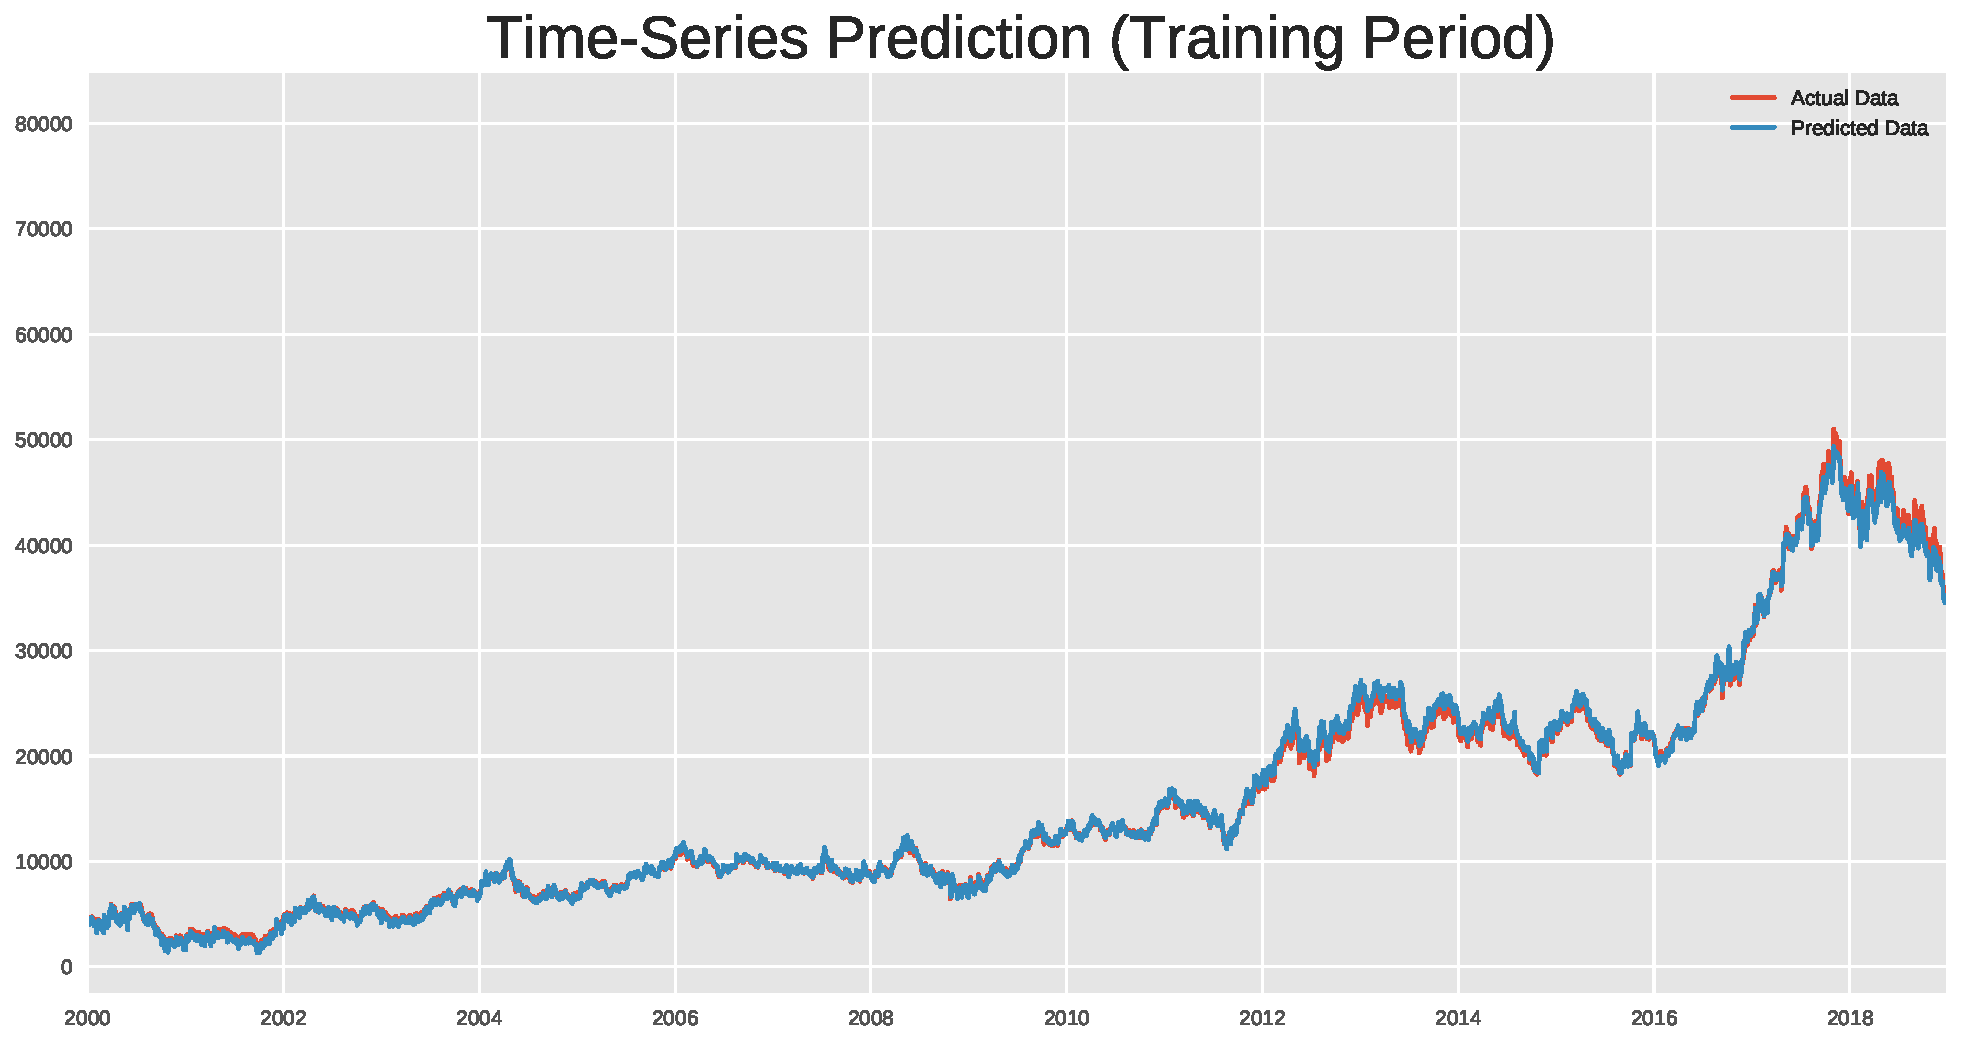
\includegraphics[width=\textwidth]{images/prediction_base_train.pdf}
    \caption{Actual and predicted adjusted closing price of Samsung's stocks the next day for the training period}
    \label{fig:train}
\end{figure}
\begin{figure}
    \centering
    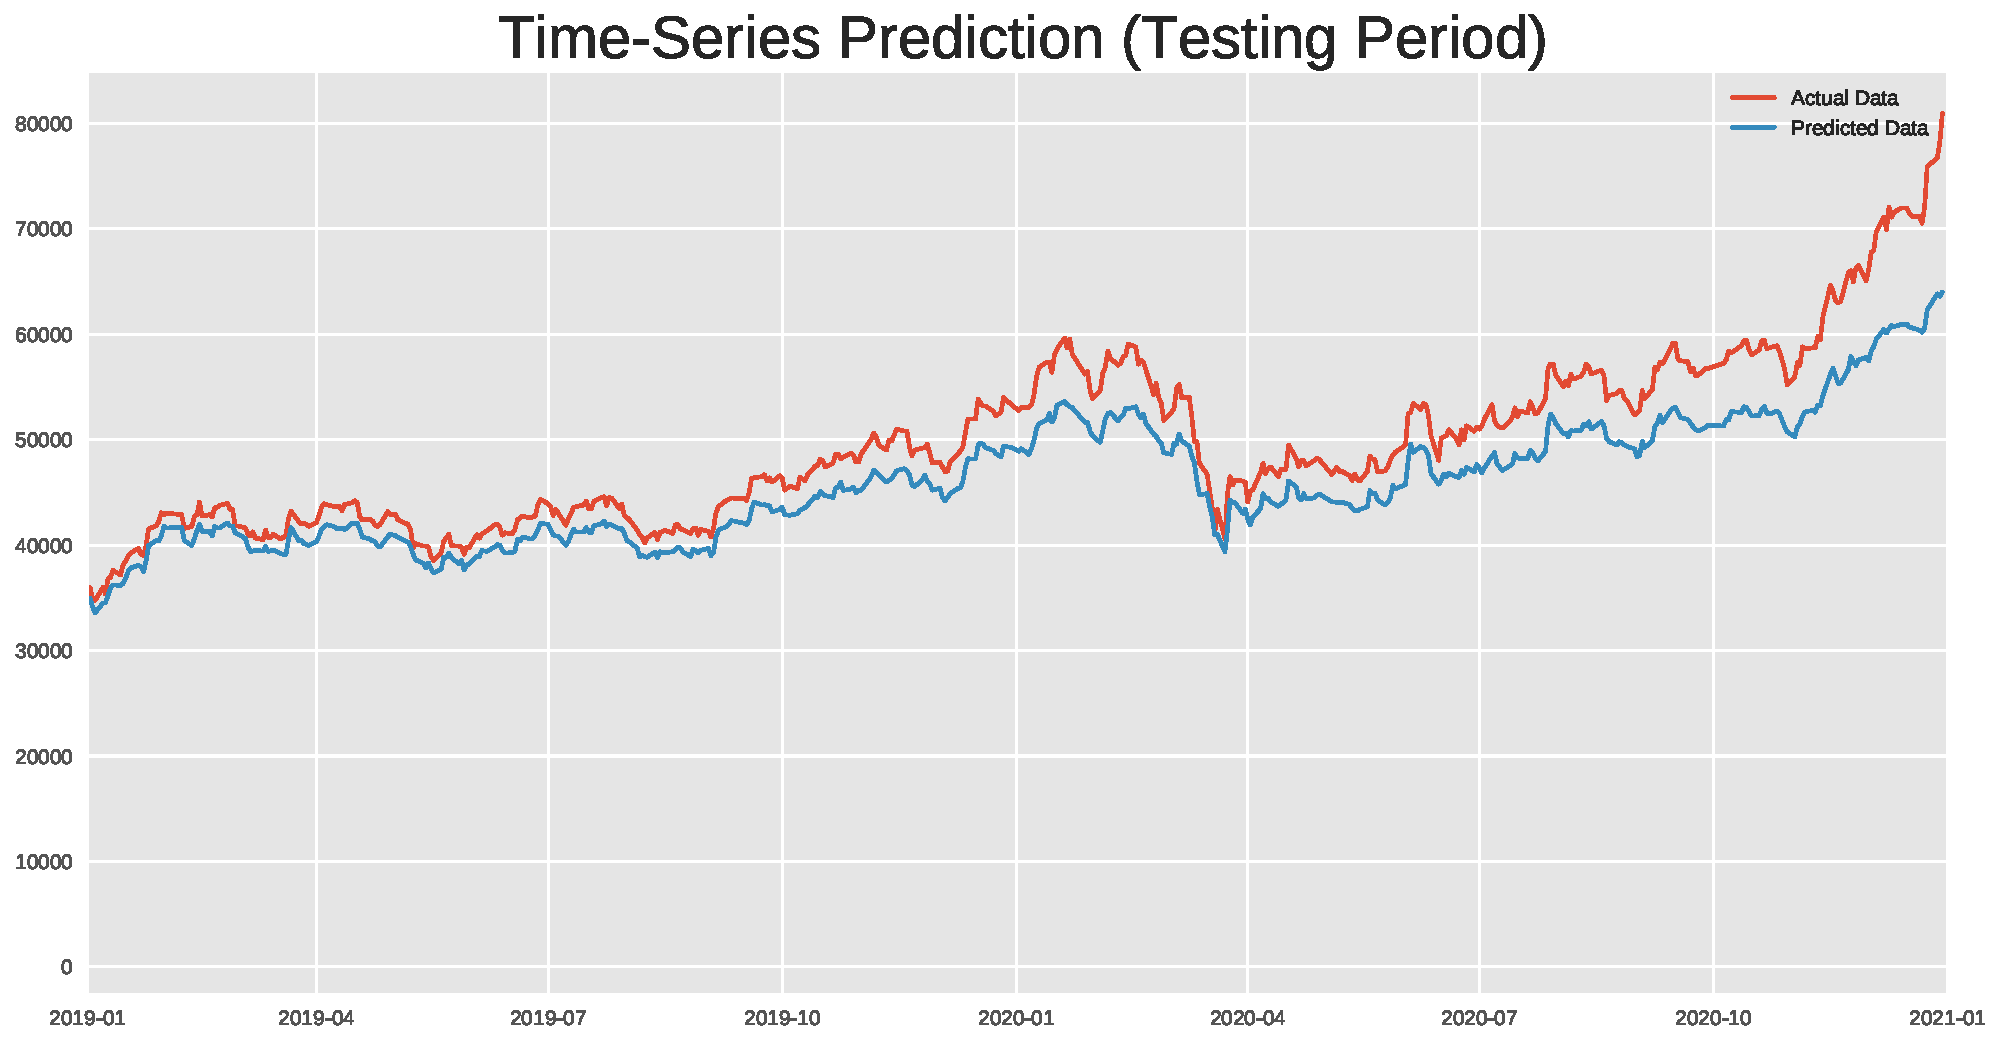
\includegraphics[width=\textwidth]{images/prediction_base_test.pdf}
    \caption{Actual and predicted adjusted closing price of the next day for the test period}
    \label{fig:test}
\end{figure}
\paragraph{5.} \textit{Comparison of the test and training set}. We can see from Figure \ref{fig:test} that the model has been properly fitted, which can be also seen in the loss of Table \ref{tab:loss}. The test set in Figure \ref{fig:test} shows that the model is still able to predict \textit{well} unseen data, even though the gap between actual and predicted data grows wider at the end of 2020. This may also be due to unseen events, i.e. the COVID-19 pandemic.

\paragraph{6.} \textit{Mean Squared Error for both predicted and test data}. The Mean Squared Error (MSE) can be written as:
\begin{equation}
    MSE = \frac{1}{n} \sum_{i=1}^n (y_i - \hat{y}_i)^2
\end{equation}
where $n$ is the number of data points, $y_i$ are the actual values and $\hat{y}_i$ are the predicted ones.
The values obtained are the following:
\begin{center}
\rowcolors{2}{gray!25}{white}     
    \begin{tabular}{l rl}
    \rowcolor{gray!50}
         &  \textbf{MSE}\\
         \hline
         \text{Training Data} & 234,280.4\\
         \text{Test Data} & 18,589,588.0 \\
    \end{tabular}
\end{center}

\subsection{Predicting Microsoft's stock price}
We will extend the experiments with LSTM by predicting the Microsoft Corporation stock price \footnote{Source: \href{https://finance.yahoo.com/quote/MSFT/}{Yahoo Finance}}.
As we can see in Figure \ref{fig:all_microsoft}, the network was able to fit well the training data, while in the test region of \ref{fig:test_microsoft} it shows comparable results to Samsung's stock price behavior, which may be due to the COVID-19 era.

\begin{figure}
    \centering
    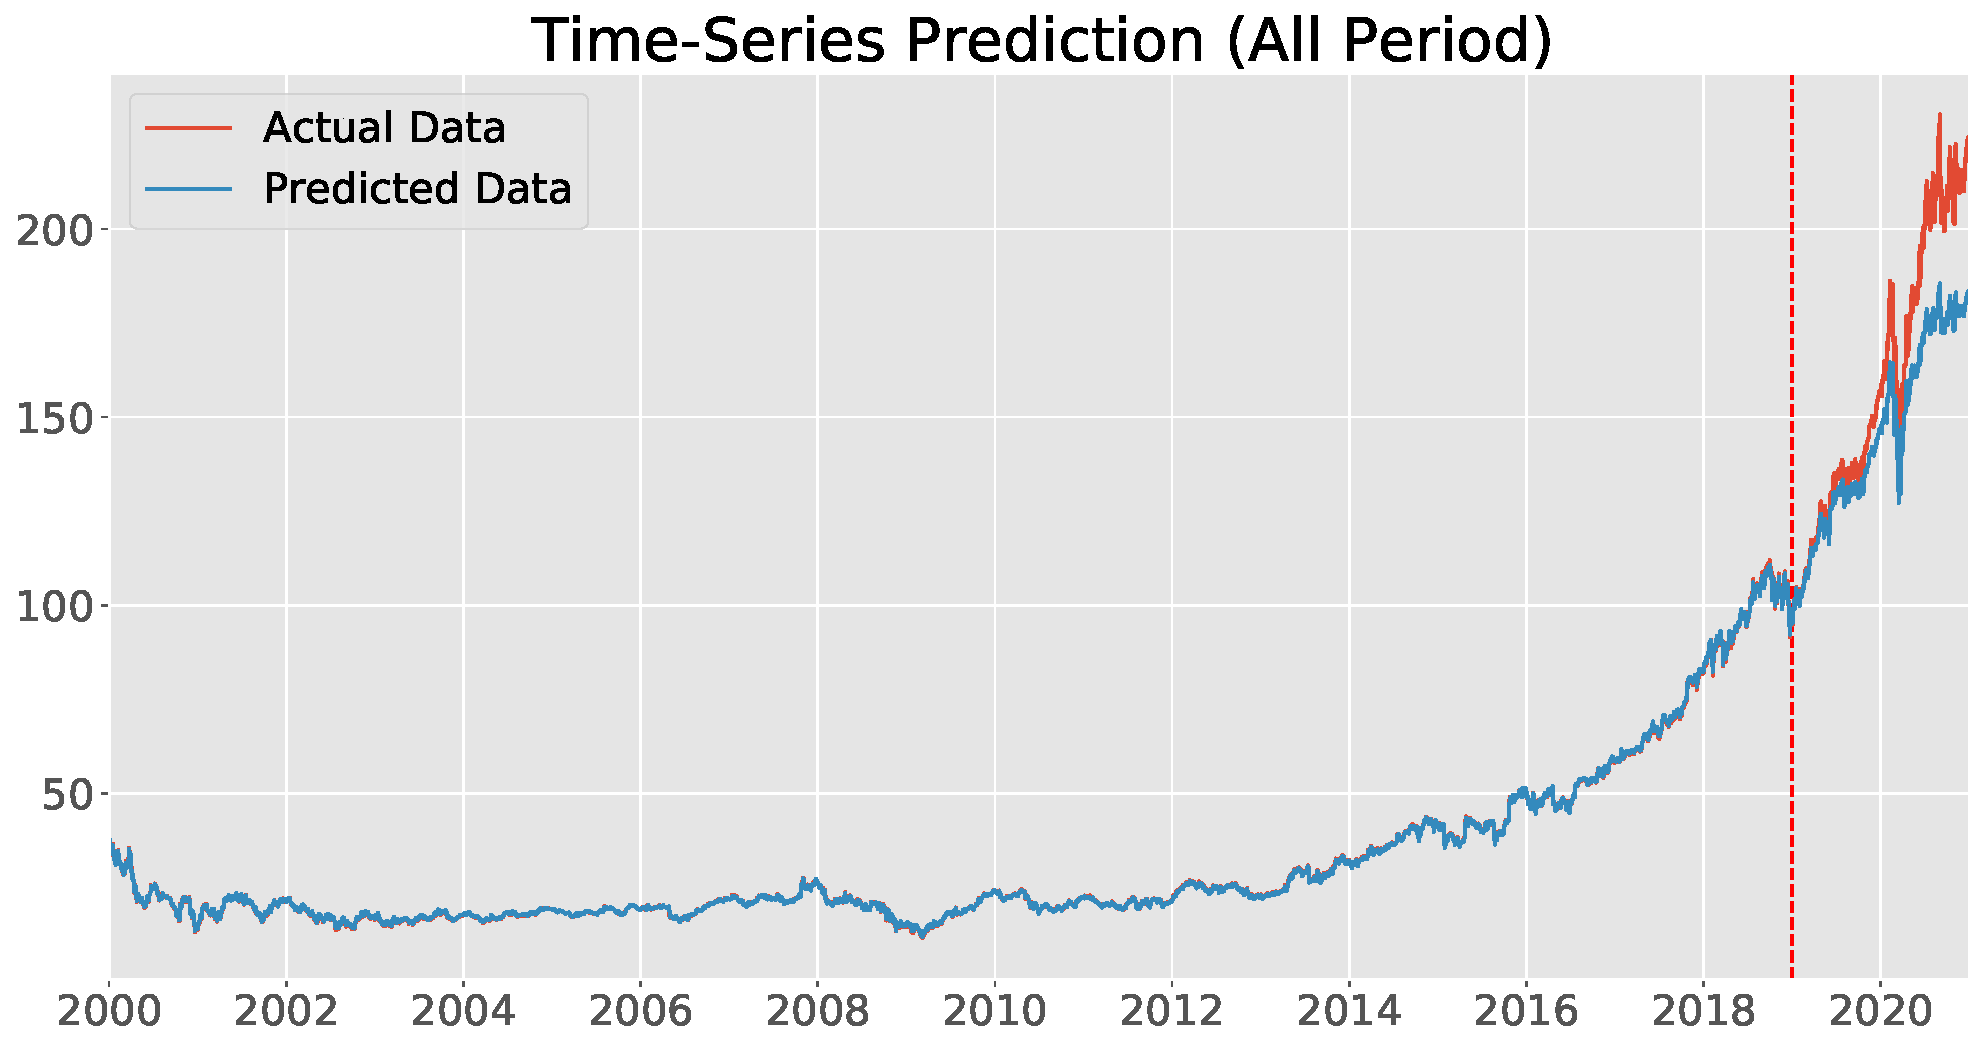
\includegraphics[width=\textwidth]{images/prediction_base_all_microsoft.pdf}
    \caption{Actual and predicted adjusted closing price of Samsung's stocks the next day for all the time period}
    \label{fig:all_microsoft}
\end{figure}
\begin{figure}
    \centering
    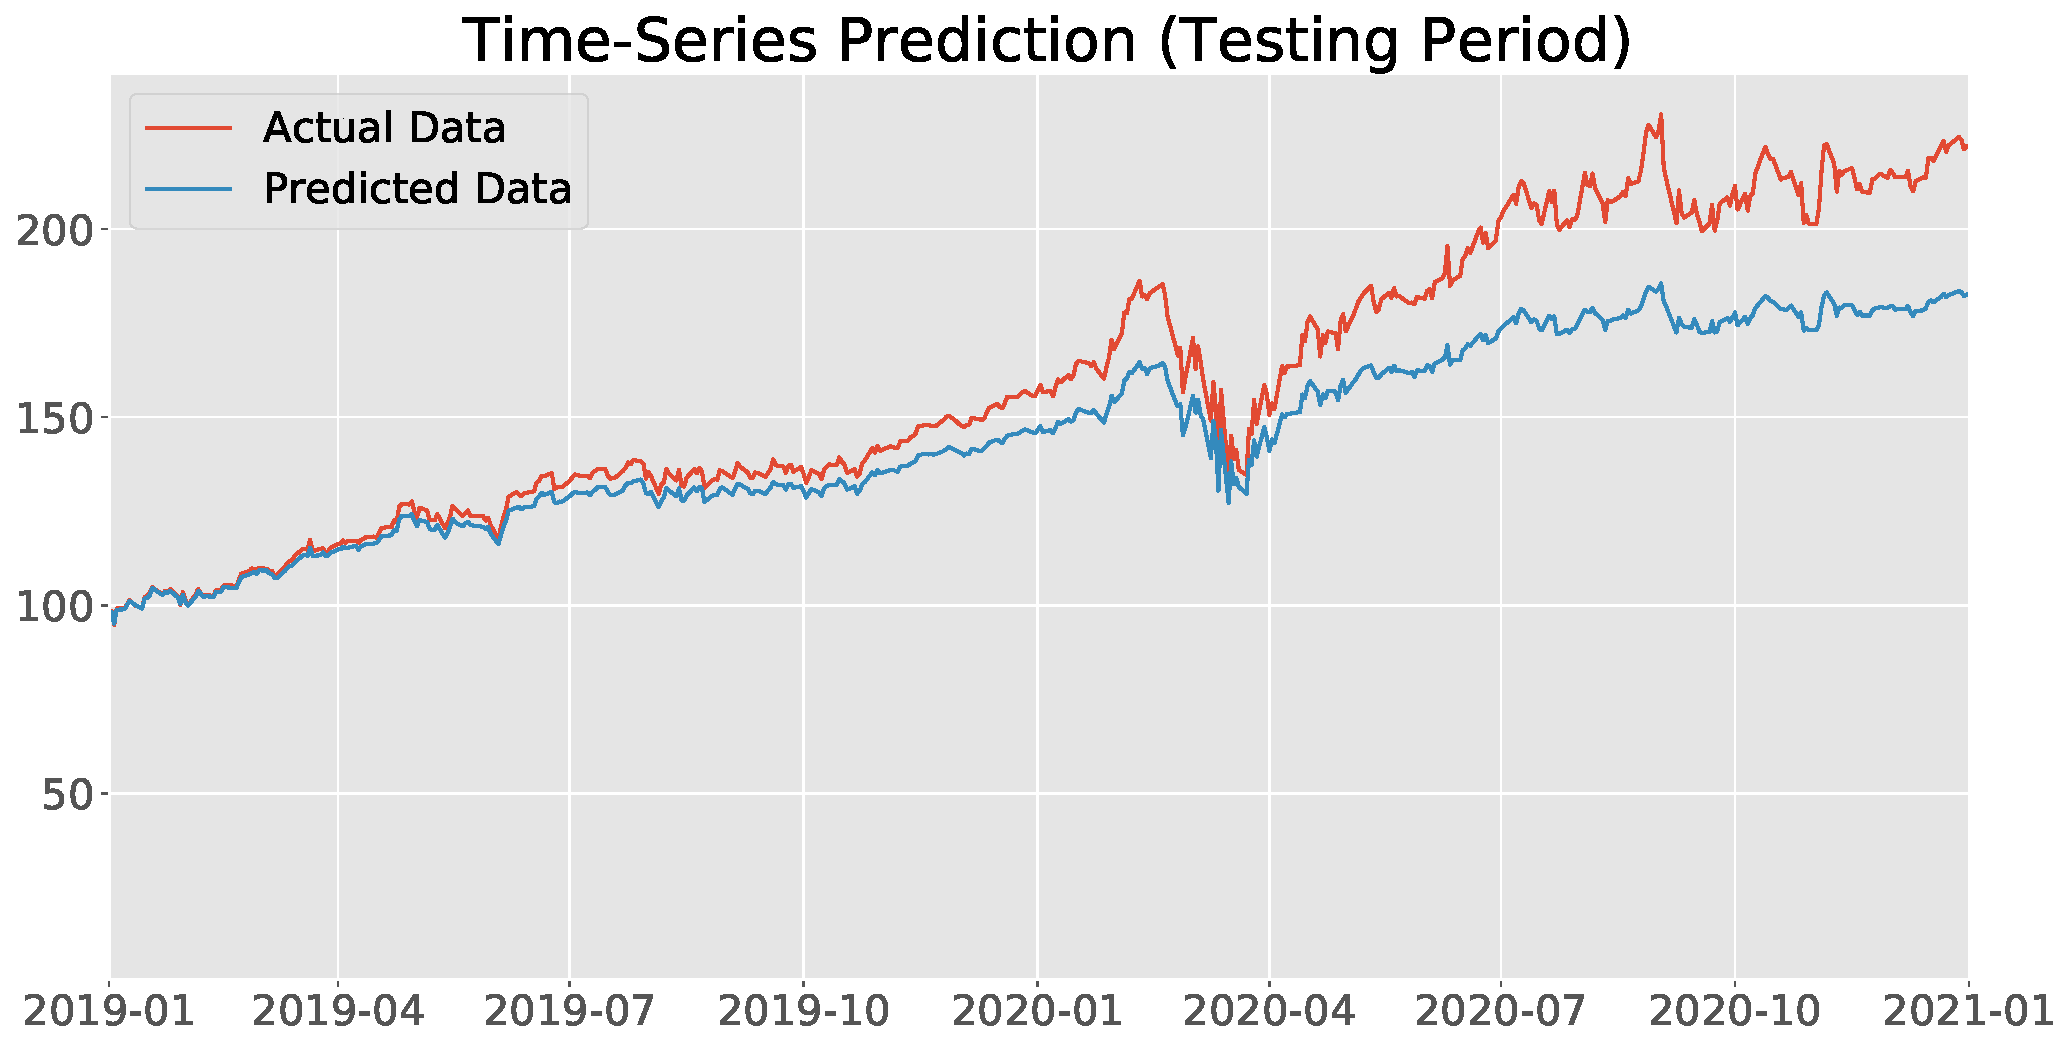
\includegraphics[width=\textwidth]{images/prediction_base_test_microsoft.pdf}
    \caption{Actual and predicted adjusted closing price of Microsoft's stocks the next day for all the test period}
    \label{fig:test_microsoft}
\end{figure}

\subsection{Predicting Tesla's stock price}
As another extension, we predict the Tesla Inc. stock price \footnote{Source: \href{https://finance.yahoo.com/quote/TSLA/}{Yahoo finance}}. 
This dataset is different from the previous two since it starts in 2010 and we made the prediction up to April 2021.
Figure \ref{fig:all_tesla} shows that the LSTM could fit very well the training set, while Figure \ref{fig:test_tesla} clearly shows the network could not predict the stock price at all due to overfitting to values lower than around 200. Moreover, the COVID-19 era, coupled with the rising of Elon Musk's projects i.e. SpaceX and Gigafactory just to cite two, may be responsible for the skyrocketing of Tesla's stock prices.
\begin{figure}
    \centering
    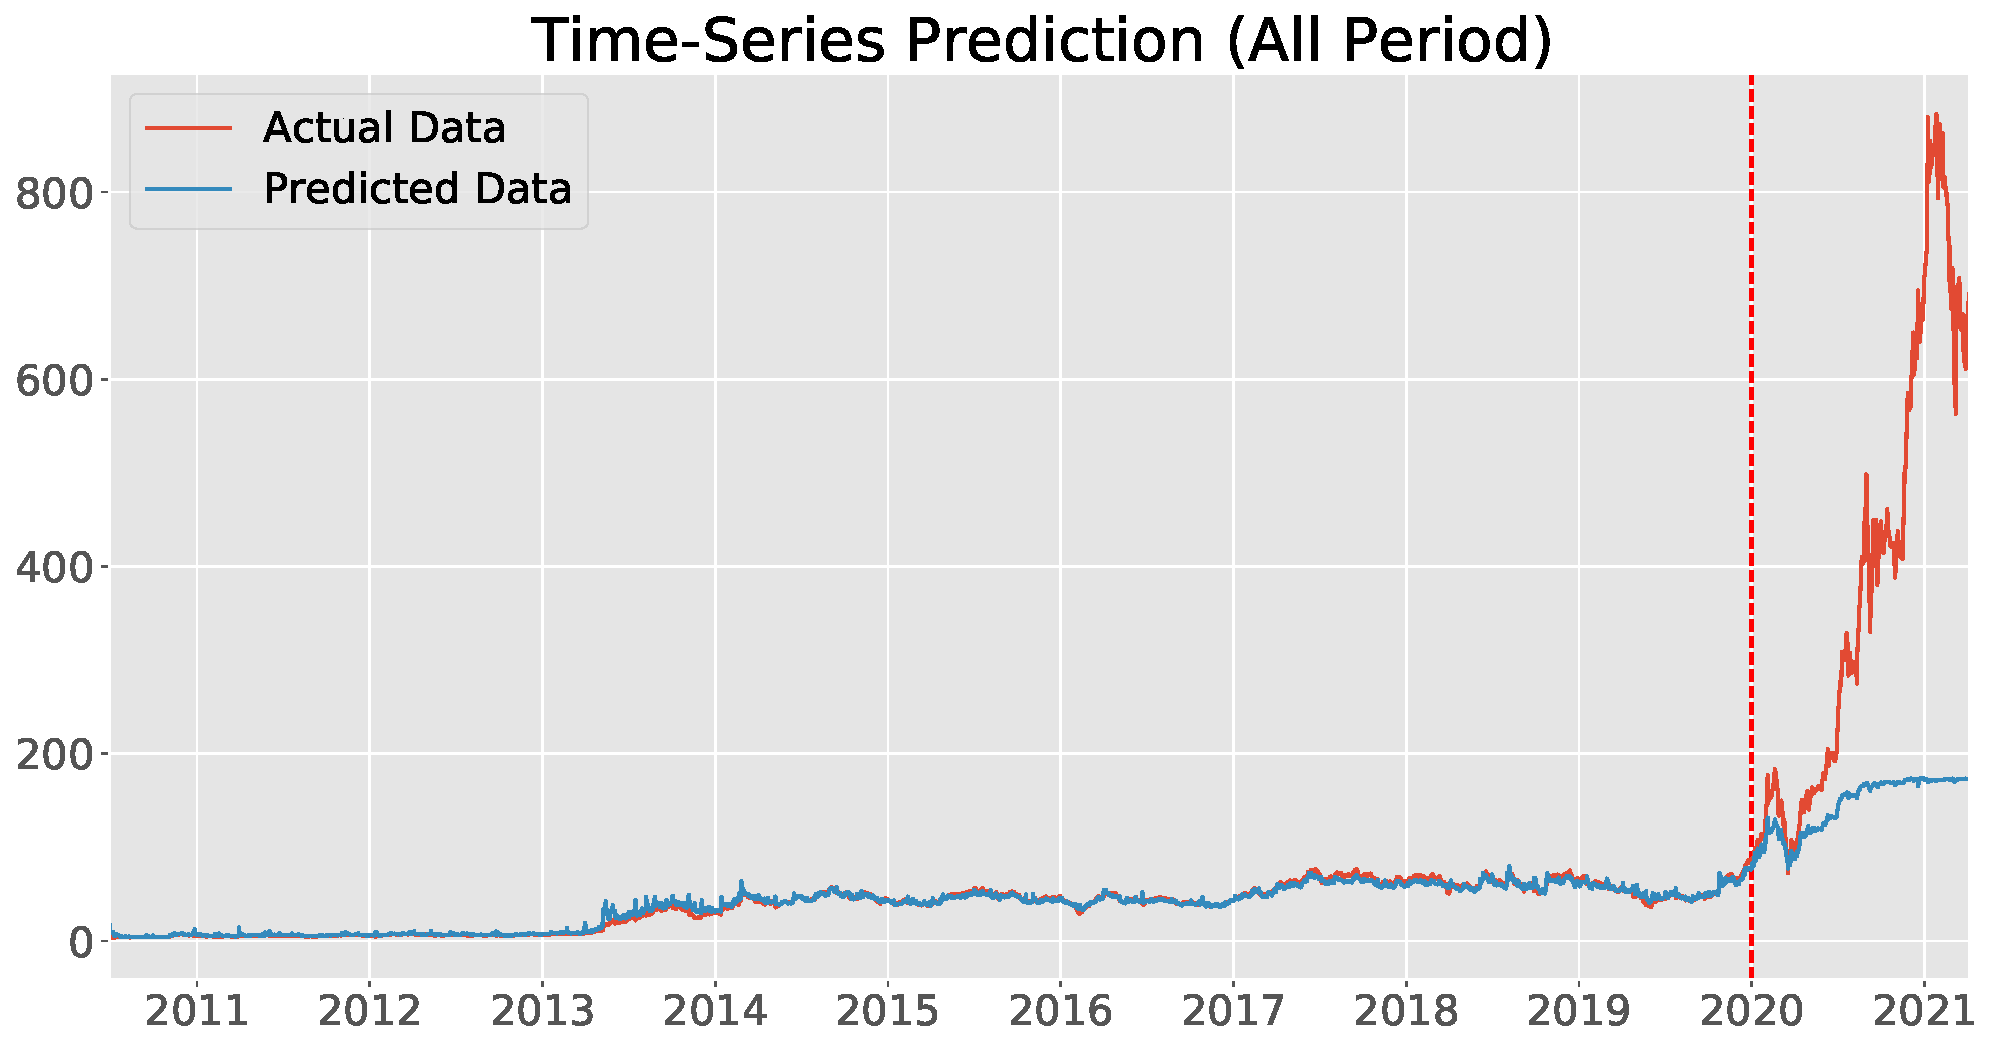
\includegraphics[width=\textwidth]{images/prediction_base_all_tesla.pdf}
    \caption{Actual and predicted adjusted closing price of Tesla's stocks the next day for the whole period}
    \label{fig:all_tesla}
\end{figure}
\begin{figure}
    \centering
    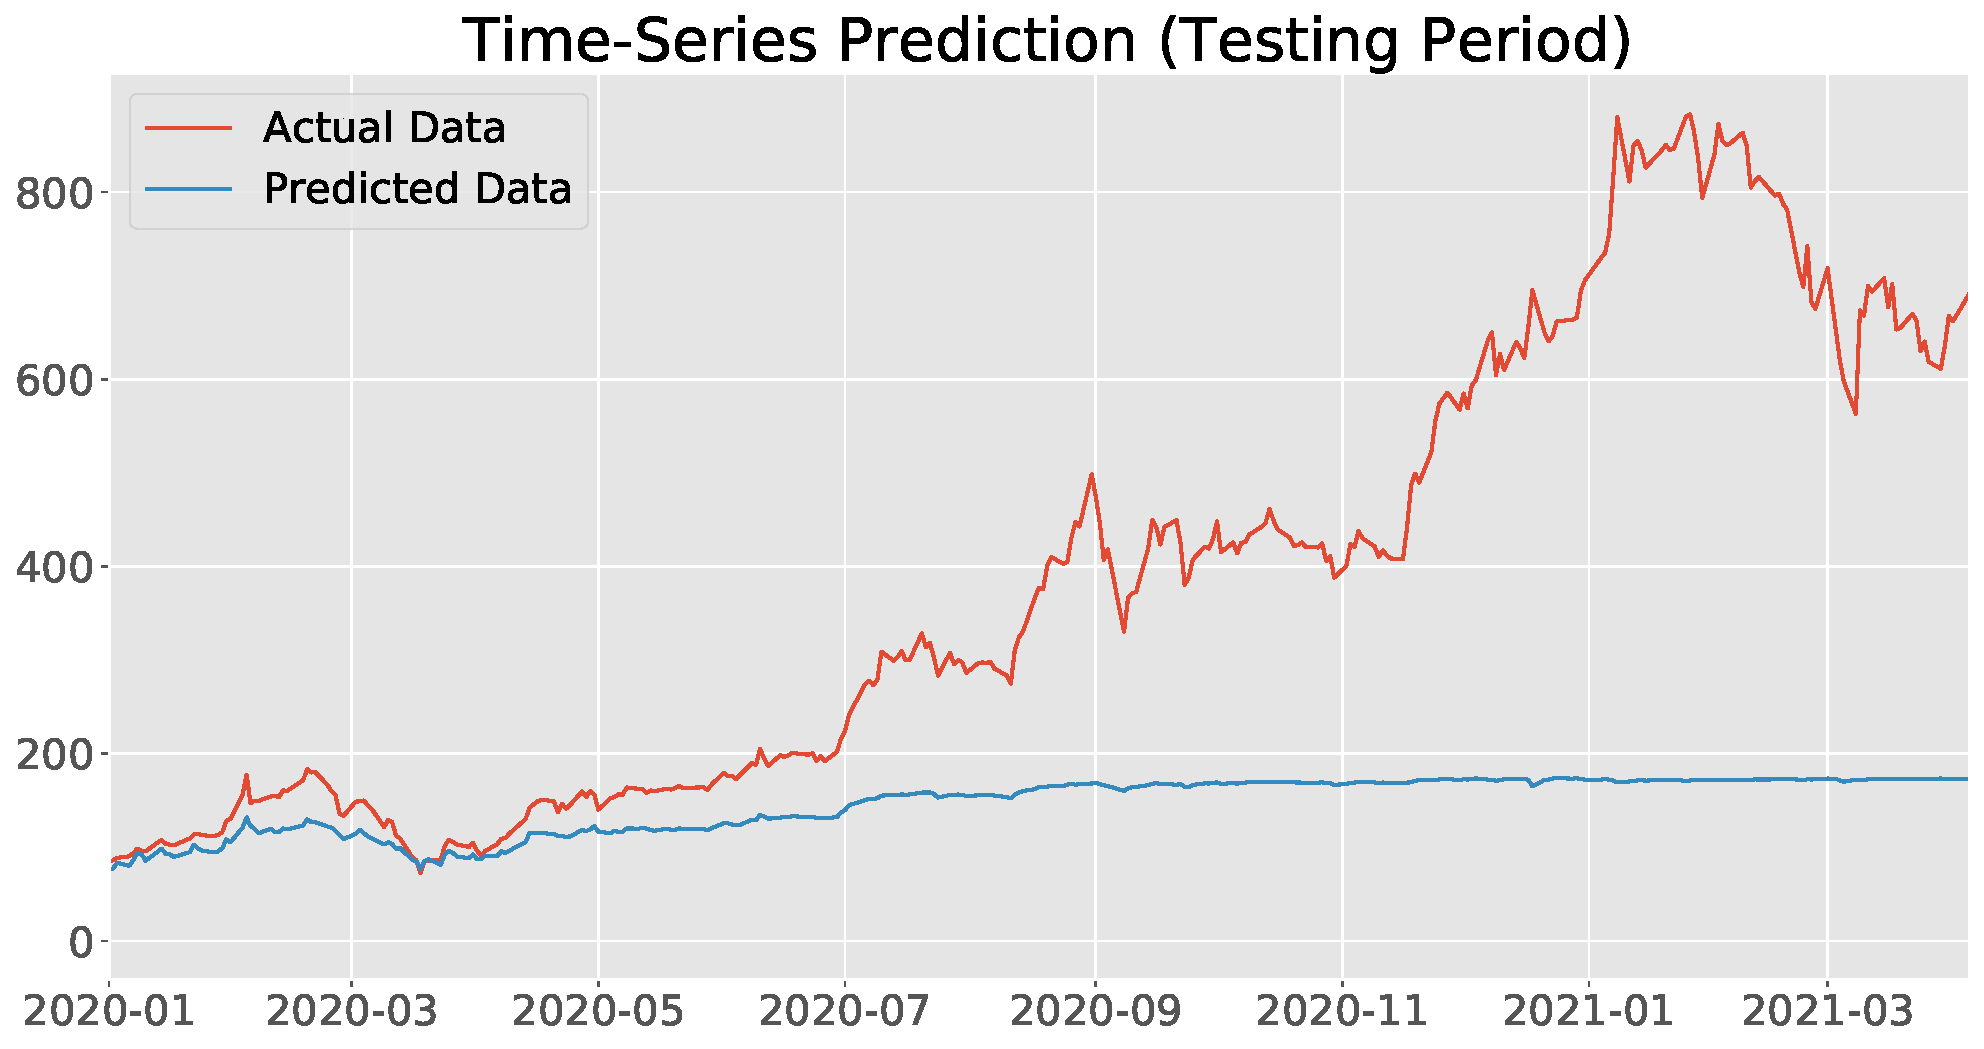
\includegraphics[width=\textwidth]{images/prediction_base_test_tesla.pdf}
    \caption{Actual and predicted adjusted closing price of Tesla's stocks the next day for the test period. The network is not able to predict well past 2020 due to the skyrocketing of stock prices which were unseen in the training set}
    \label{fig:test_tesla}
\end{figure}

\section{Improving the Predictions}
In this section, we show how to improve the algorithm in three ways:
\begin{enumerate}
    \item Revising the codes with Pytorch Lightning
    \item Using a different AI algorithm, namely Gated Recurrent Unit (GRU)
    \item Improving the MSE error results
\end{enumerate}

\subsection{Using Pytorch Lightning}
We revise the code by using Pytorch Lightning \cite{falcon2019pytorch}: this PyTorch framework provides a high-level interface by which it is easier to control architectures, results, logging and more. 
More importantly, it makes the process of moving models to GPU, Tensor Processing Units (TPUs) and even multiple GPUs and TPUs easier while having a negligible overhead. This open-source library is actively maintained by a community highly focused on efficiency and code readability. We refactor the code to be used with Pytorch Lightning.

\subsection{The GRU model}
Gated Recurrent Units (GRU) \cite{cho2014learning} were proposed as an RNN variant in 2014: they are similar to LSTMs without an output gate and has fewer parameters. Figure \ref{fig:gru} shows an overview of the architecture.
\begin{figure}[h!]
    \centering
    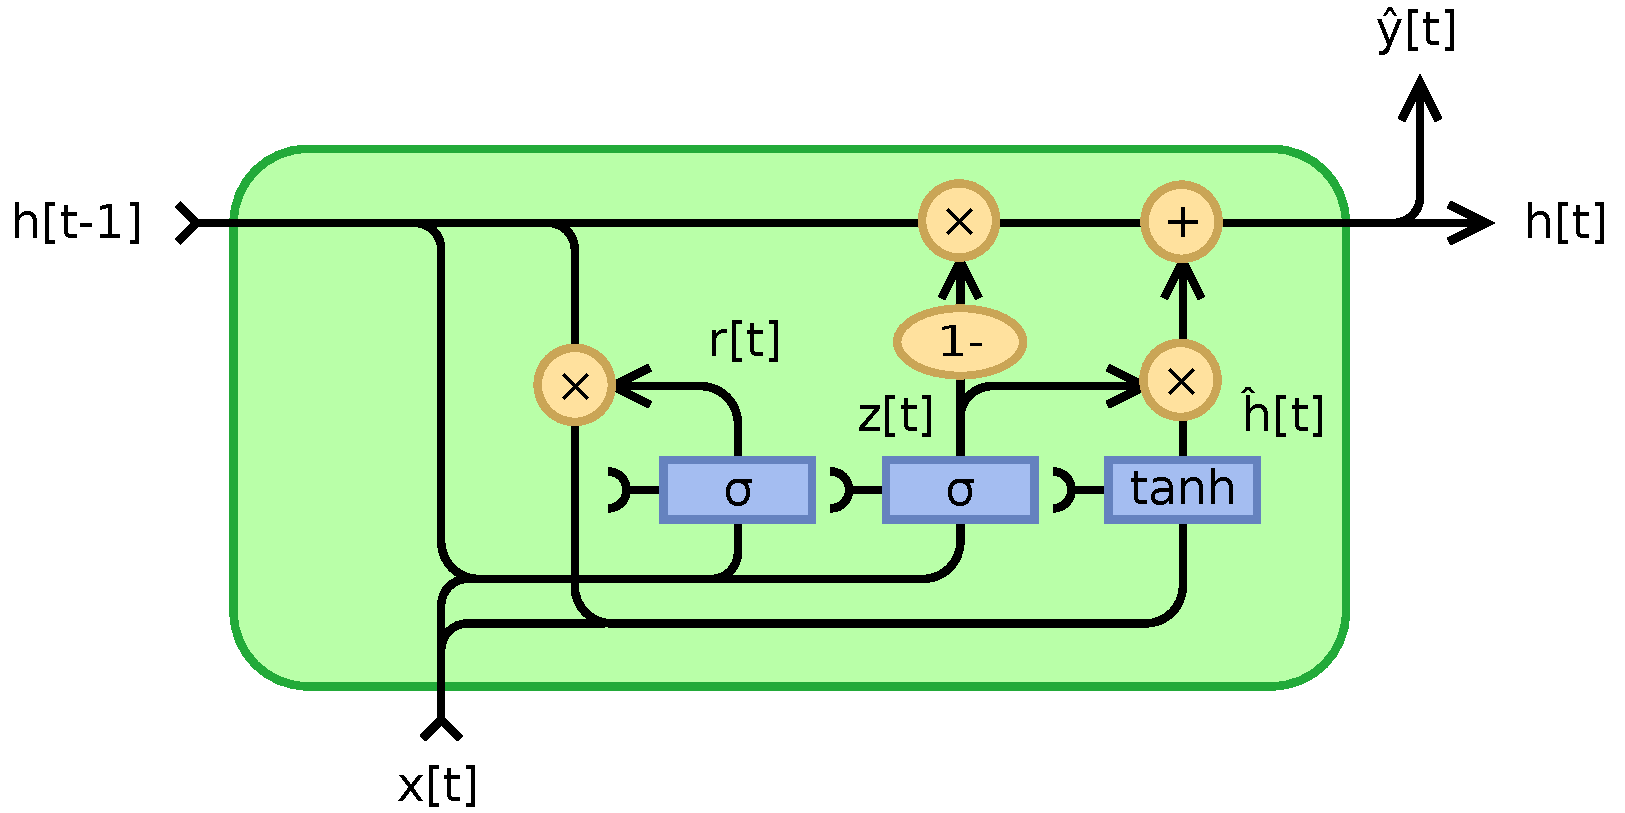
\includegraphics[width=0.7\linewidth]{images/Gated_Recurrent_Unit,_base_type.pdf}
    \caption{Gated Recurrent Unit (GRU) base model}
    \label{fig:gru}
\end{figure}
Having fewer parameters than LSTM, GRUs have been shown to perform better on certain dataset and have better generalization capabilities with fewer data.

\subsection{Predicting Samsung's stocks with GRU}
We implement GRU on the same dataset as the one used with LSTM. Figure \ref{fig:gru_all} shows that GRU successfully fits the training dataset and the predicted values are close to the actual ones.
\begin{figure}
    \centering
    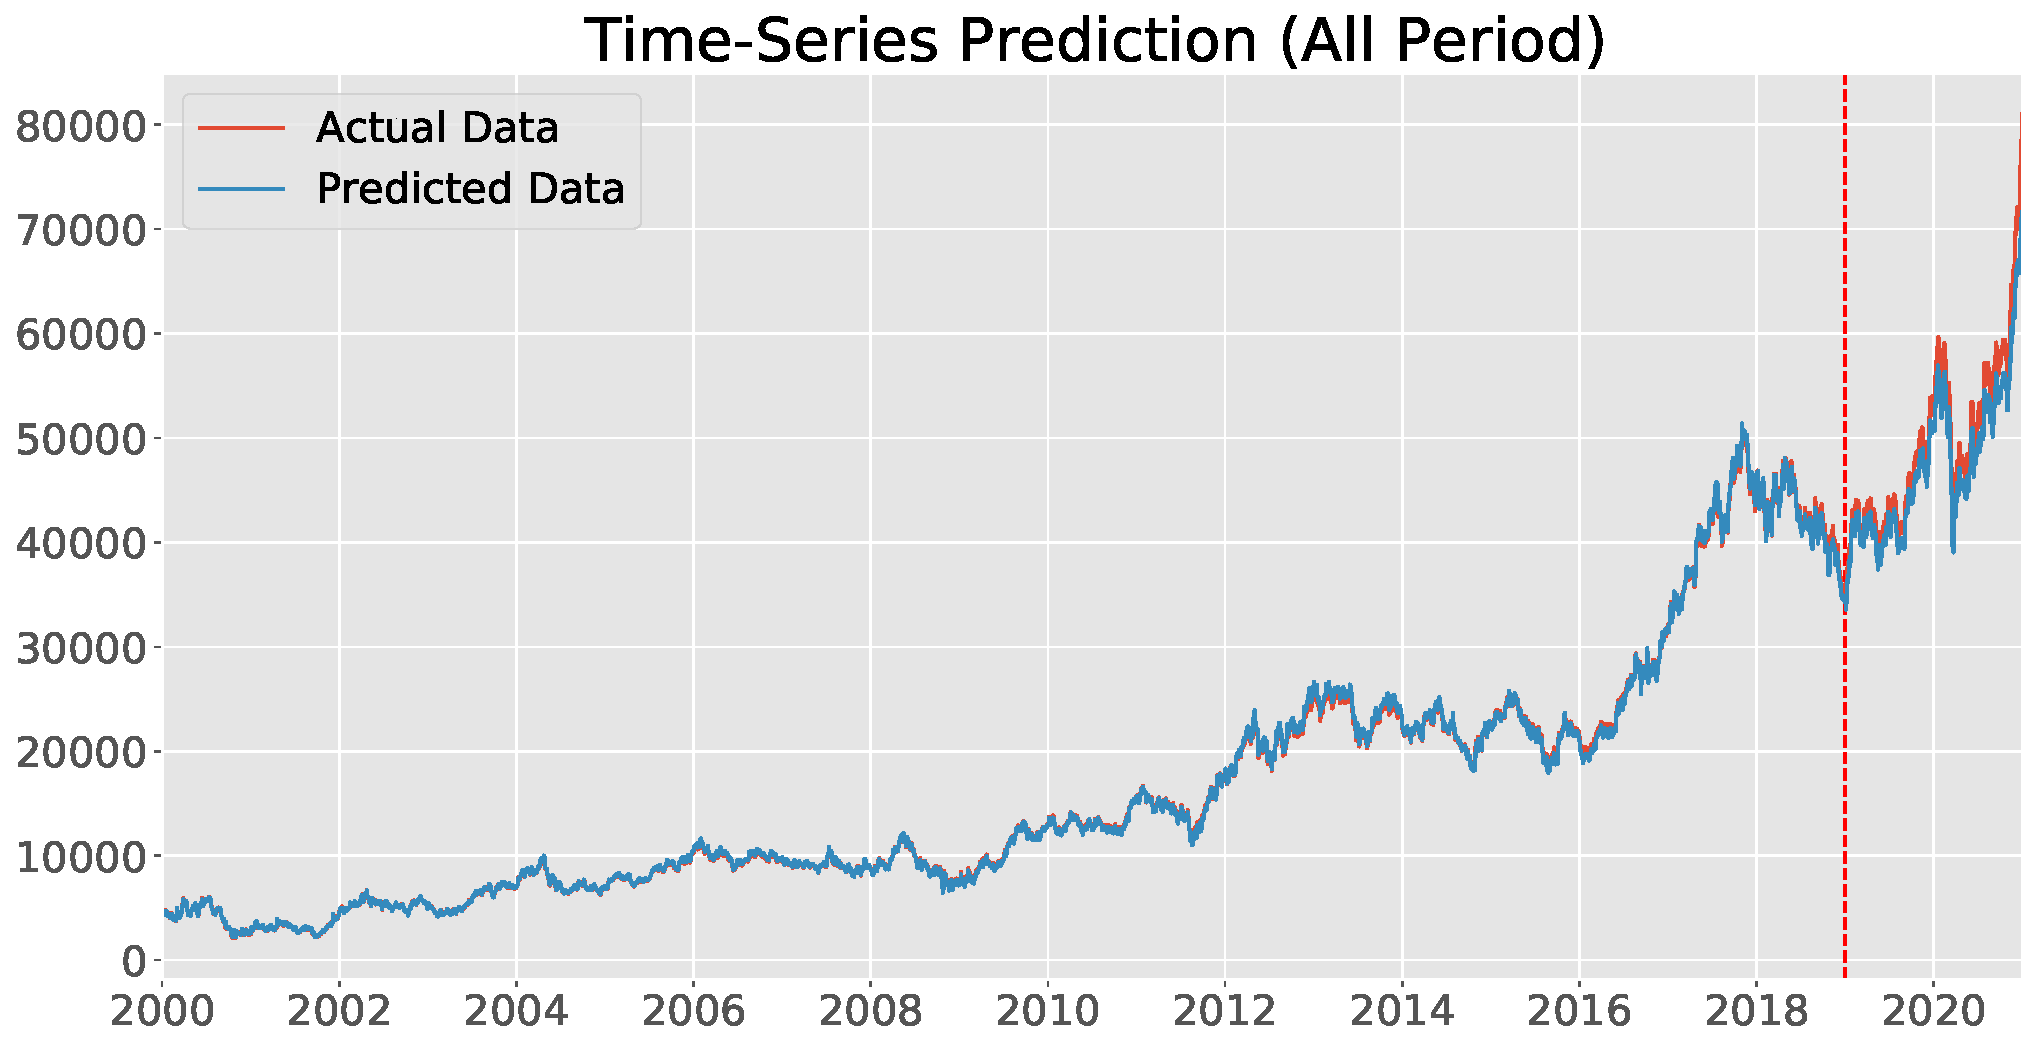
\includegraphics[width=\linewidth]{images/prediction_base_all_gru.pdf}
    \caption{Actual and GRU-predicted adjusted closing price of Samsung's stocks the next day for the whole period}
    \label{fig:gru_all}
\end{figure}

\subsection{Comparing LSTM and GRU}
\subsubsection{Samsung's stock price}
We show in the Table \ref{tab:lstm_gru} the results of the MSE, while Figure \ref{fig:lstm_vs_gru_all} we compare the results graphically.

\begin{center}
\rowcolors{2}{gray!25}{white}
\label{tab:lstm_gru}
    \begin{tabular}{l rl rl}
    \rowcolor{gray!50}
         &  \textbf{LSTM - MSE} & \textbf{GRU - MSE}\\
         \hline
         \text{Training Data} & 234,280.4 & 51,174.5\\
         \text{Test Data} & 18,589,588.0 & 5,497,948.0\\
    \end{tabular}
\end{center}

\begin{figure}
    \centering
    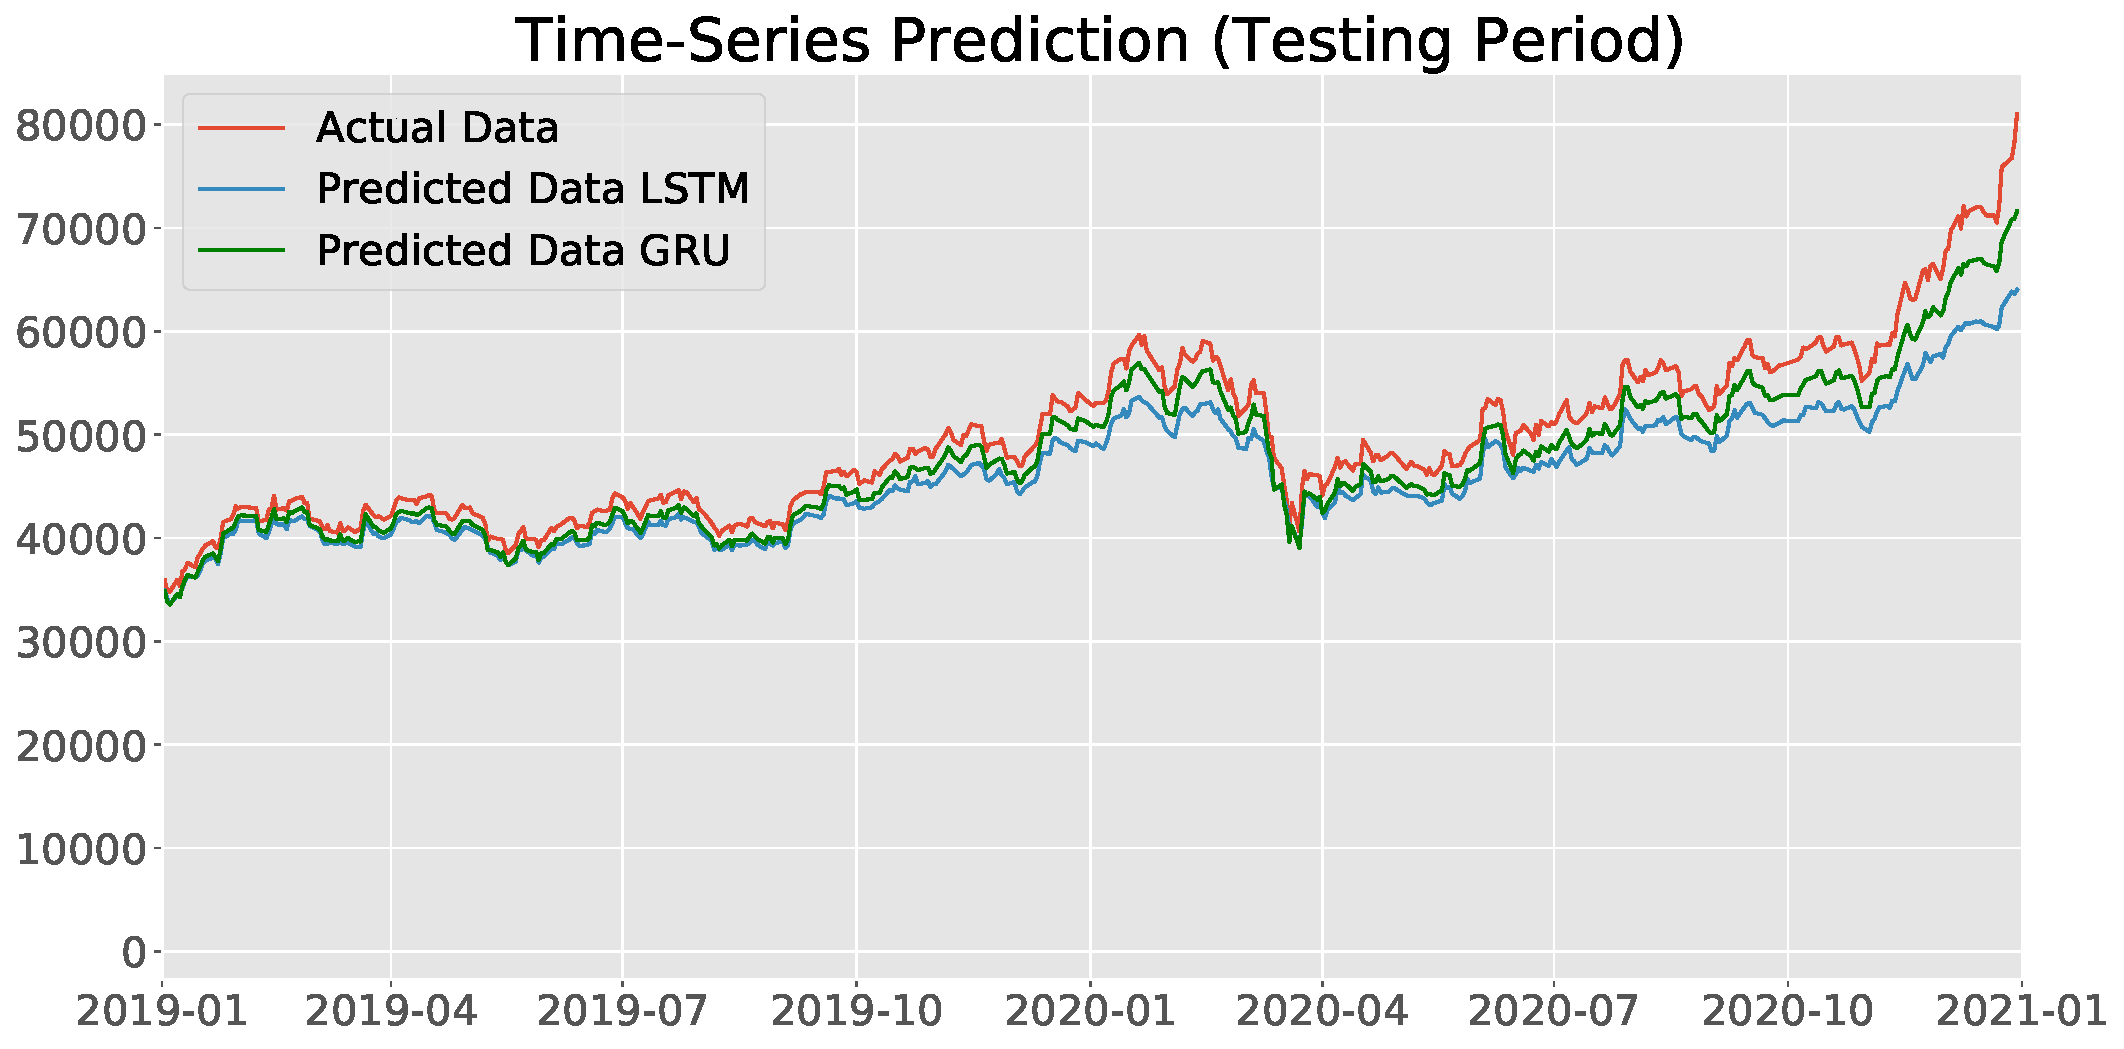
\includegraphics[width=\linewidth]{images/prediction_base_test_lstm_gru.pdf}
    \caption{Actual, LSTM-predicted and GRU-predicted adjusted closing price of Samsung's stocks the next day for the test period. GRU has better generalization properties on this dataset.}
    \label{fig:lstm_vs_gru_all}
\end{figure}

As we can see, GRU is able to achieve better results than LSTM, which we confirmed with multiple experiments as well. As suggested in the seminal paper, this could be due to less parameters which guarantee better generalization properties when compared to LSTM; especially considering the fact that the dataset provided is not high-dimensional.

\subsubsection{Tesla's stock price}

\begin{figure}
    \centering
    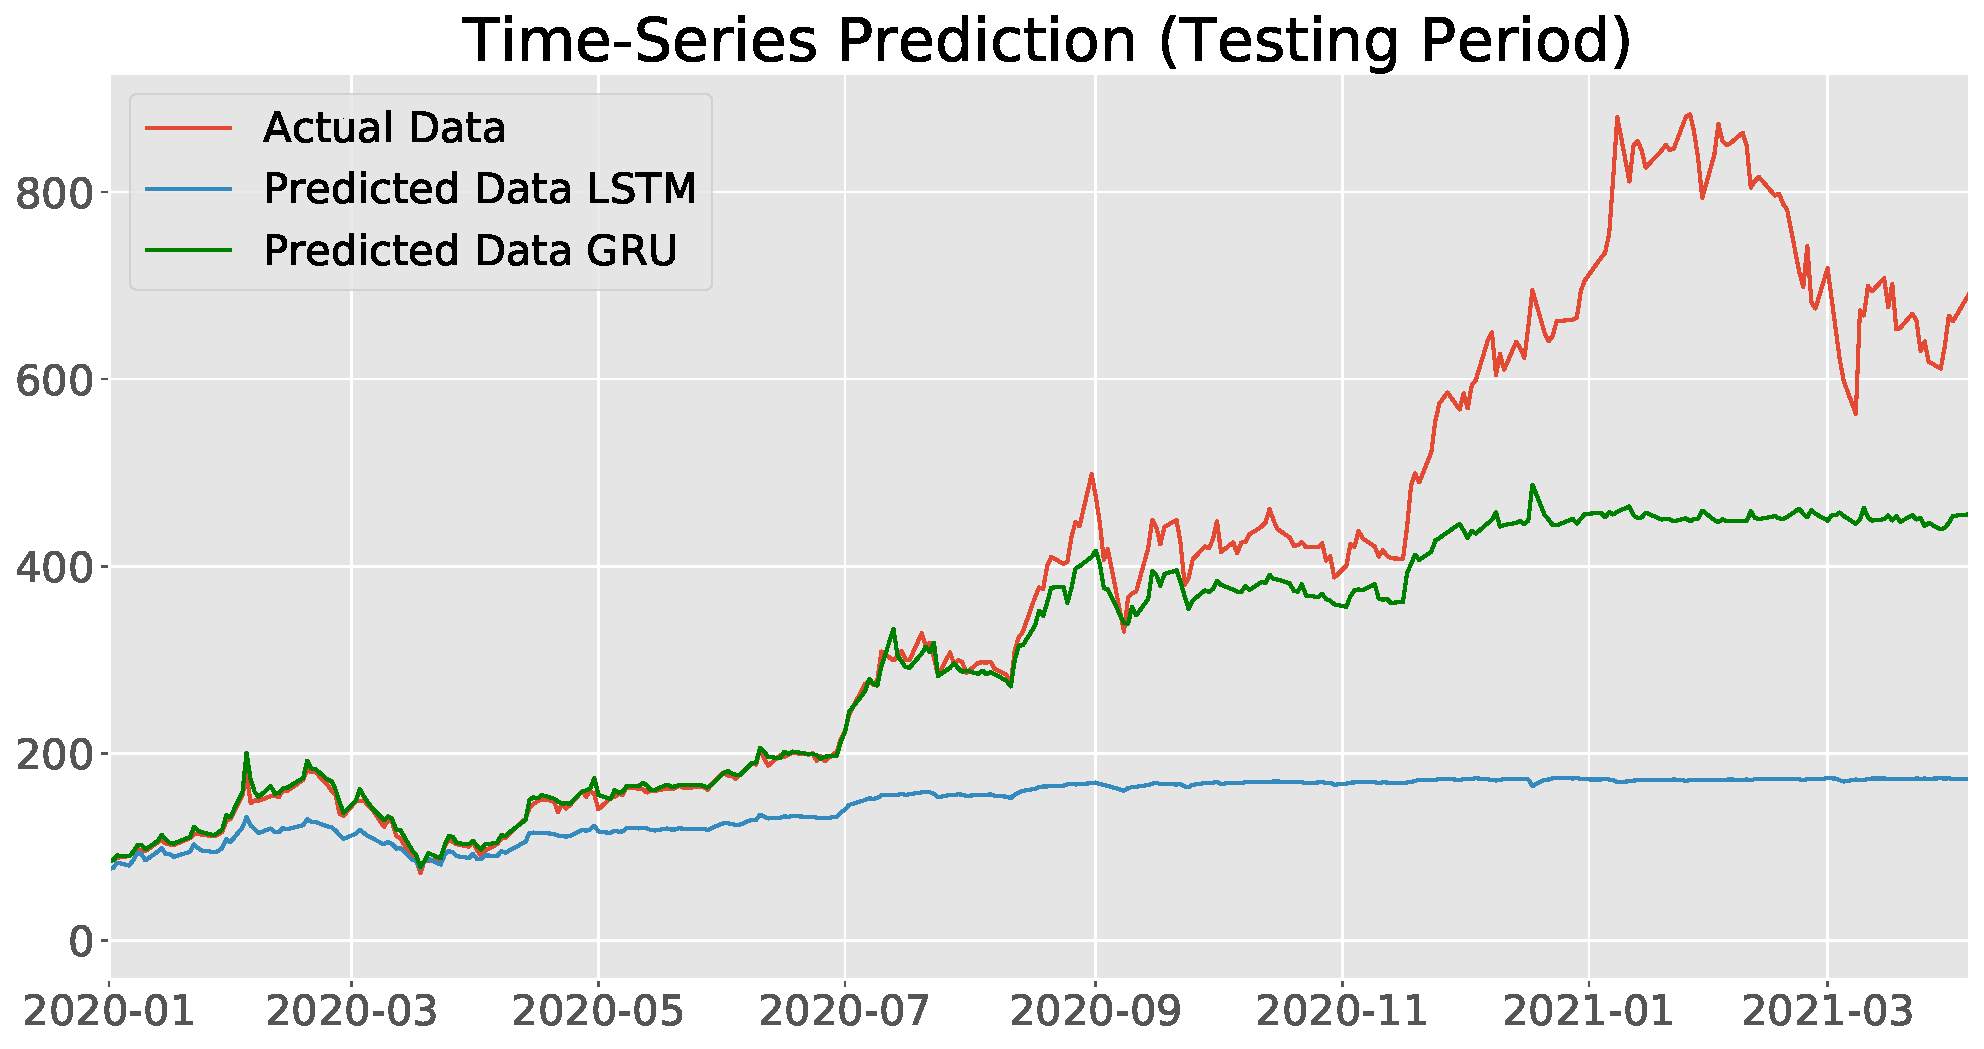
\includegraphics[width=\linewidth]{images/prediction_test_lstm_gru_tesla.pdf}
    \caption{Actual, LSTM-predicted and GRU-predicted adjusted closing price of Tesla's stocks the next day for the test period. GRU has better generalization properties on this dataset, even though the test data differs greatly compared to the past observations due to 2020's skyrocketing of Tesla's stock prices.}
    \label{fig:lstm_vs_gru_test_tesla}
\end{figure}

We repeated the experiment of Tesla's stock prices prediction over 2020 onwards: this dataset is particularly difficult to predict due to the unseen behavior of stocks in the test set: even though LSTM achieved a good fit on the training data, it could not generalize to unseen data.
Figure \ref{fig:lstm_vs_gru_test_tesla} shows the comparisons of LSTM and GRU: while the former is not able to generalize to the unseen data and the solution diverges, GRU is able to consistently keep track of stocks behavior until around November 2020, while after that it still performs quantitatively better than LSTM.

 %%%%%%%%%% BIBLIOGRAPHY %%%%%%%%%% 
\bibliographystyle{plain}
\bibliography{ref}

\end{document}